\documentclass[../../dd.tex]{subfiles}

% Document
\begin{document}
    \chapter{Frameworks, External services and Libraries}
    \section{Framework}

    \begin{figure}[H]
        \centering
        
\includegraphics[scale=0.6]{../../assets/technology.png}
        \caption{Technological stack}\label{fig:tech-stack}
    \end{figure}

    \subsection{Flutter}
    Baddy mobile application was developed using \textbf{Flutter}, an open-source development kit created by Google used to develop applications for Android, iOS, Linux, Mac, Windows, Google from a single codebase. The main reasons of this choice are:

    \begin{itemize}
        \item \textbf{Portability}: with a single code base is possible to create a product that would fit both iOS and Android devices. Furthermore, it is possible to use it to create web and desktop apps, but these features are still under testing;
        \item \textbf{Rich in components}: Flutter has a lot of UI components that come together with the framework, without the need for installing a lot of external libraries to design interfaces;
        \item \textbf{High performance}: Flutter has very high performances thanks to how it works under the hood. It never uses web views or bridge to render the UI elements, but it uses his rendering engine, which is built mostly in C++.
    \end{itemize}

    \subsection{Node.js}

    The server side application relies on \textbf{Node.js}, an environment for server-side scripting based on JavaScript.  It’s a light, scalable, and cross-platform way to execute code. It uses an event-driven I/O model which makes it extremely efficient and makes scalable network application possible. The most important advantages we took into account for this choice are:

    \begin{itemize}
        \item code executes faster than in any other language;
        \item the ever-growing NPM (Node Package Manager) gives developers multiple tools and modules to use, thus further boosting their productivity;
        \item the single-threaded, event-driven architecture of Node.js allows it to handle multiple simultaneous connections efficiently;
    \end{itemize}

    \subsection{Firebase}
    Some particular features and functionalities are based instead on external service providers, in particular \textbf{Firebase Cloud Messaging} was used to send notifications to users' smartphones and \textbf{Firebase Cloud Storage} to upload and easily retrieve users' profile image. Firebase lets the developer to focus on developing the best app possible for the business by simplifying a lot of operations. Since the operations and internal functions are so solid, and taken care of by the Firebase interface, there is more time available for developing high quality app that users are going to want to use.


    \section{External Services}
    As already mentioned, some features of \textit{Baddy} have been implemented with the help of a series of external services. This choice comes from some simple considerations that take into account that each provider offers a consolidated platform supported by a detailed documentation and a large community of developers.
    Here are reported the external services that the application use for some of its functionalities.

    \subsection{Firebase Cloud Messaging}
    Firebase Cloud Messaging (FCM) is a platform that provides a reliable and efficient connection between servers and devices that allows to deliver and receive messages and notifications on iOS, Android, and the web at no cost. As part of the application it is used to send notifications to a caregiver's account when someone writes a review about him/her or a customer sends a message of interest after viewing his/her profile.

    \begin{figure}[H]
        \centering
        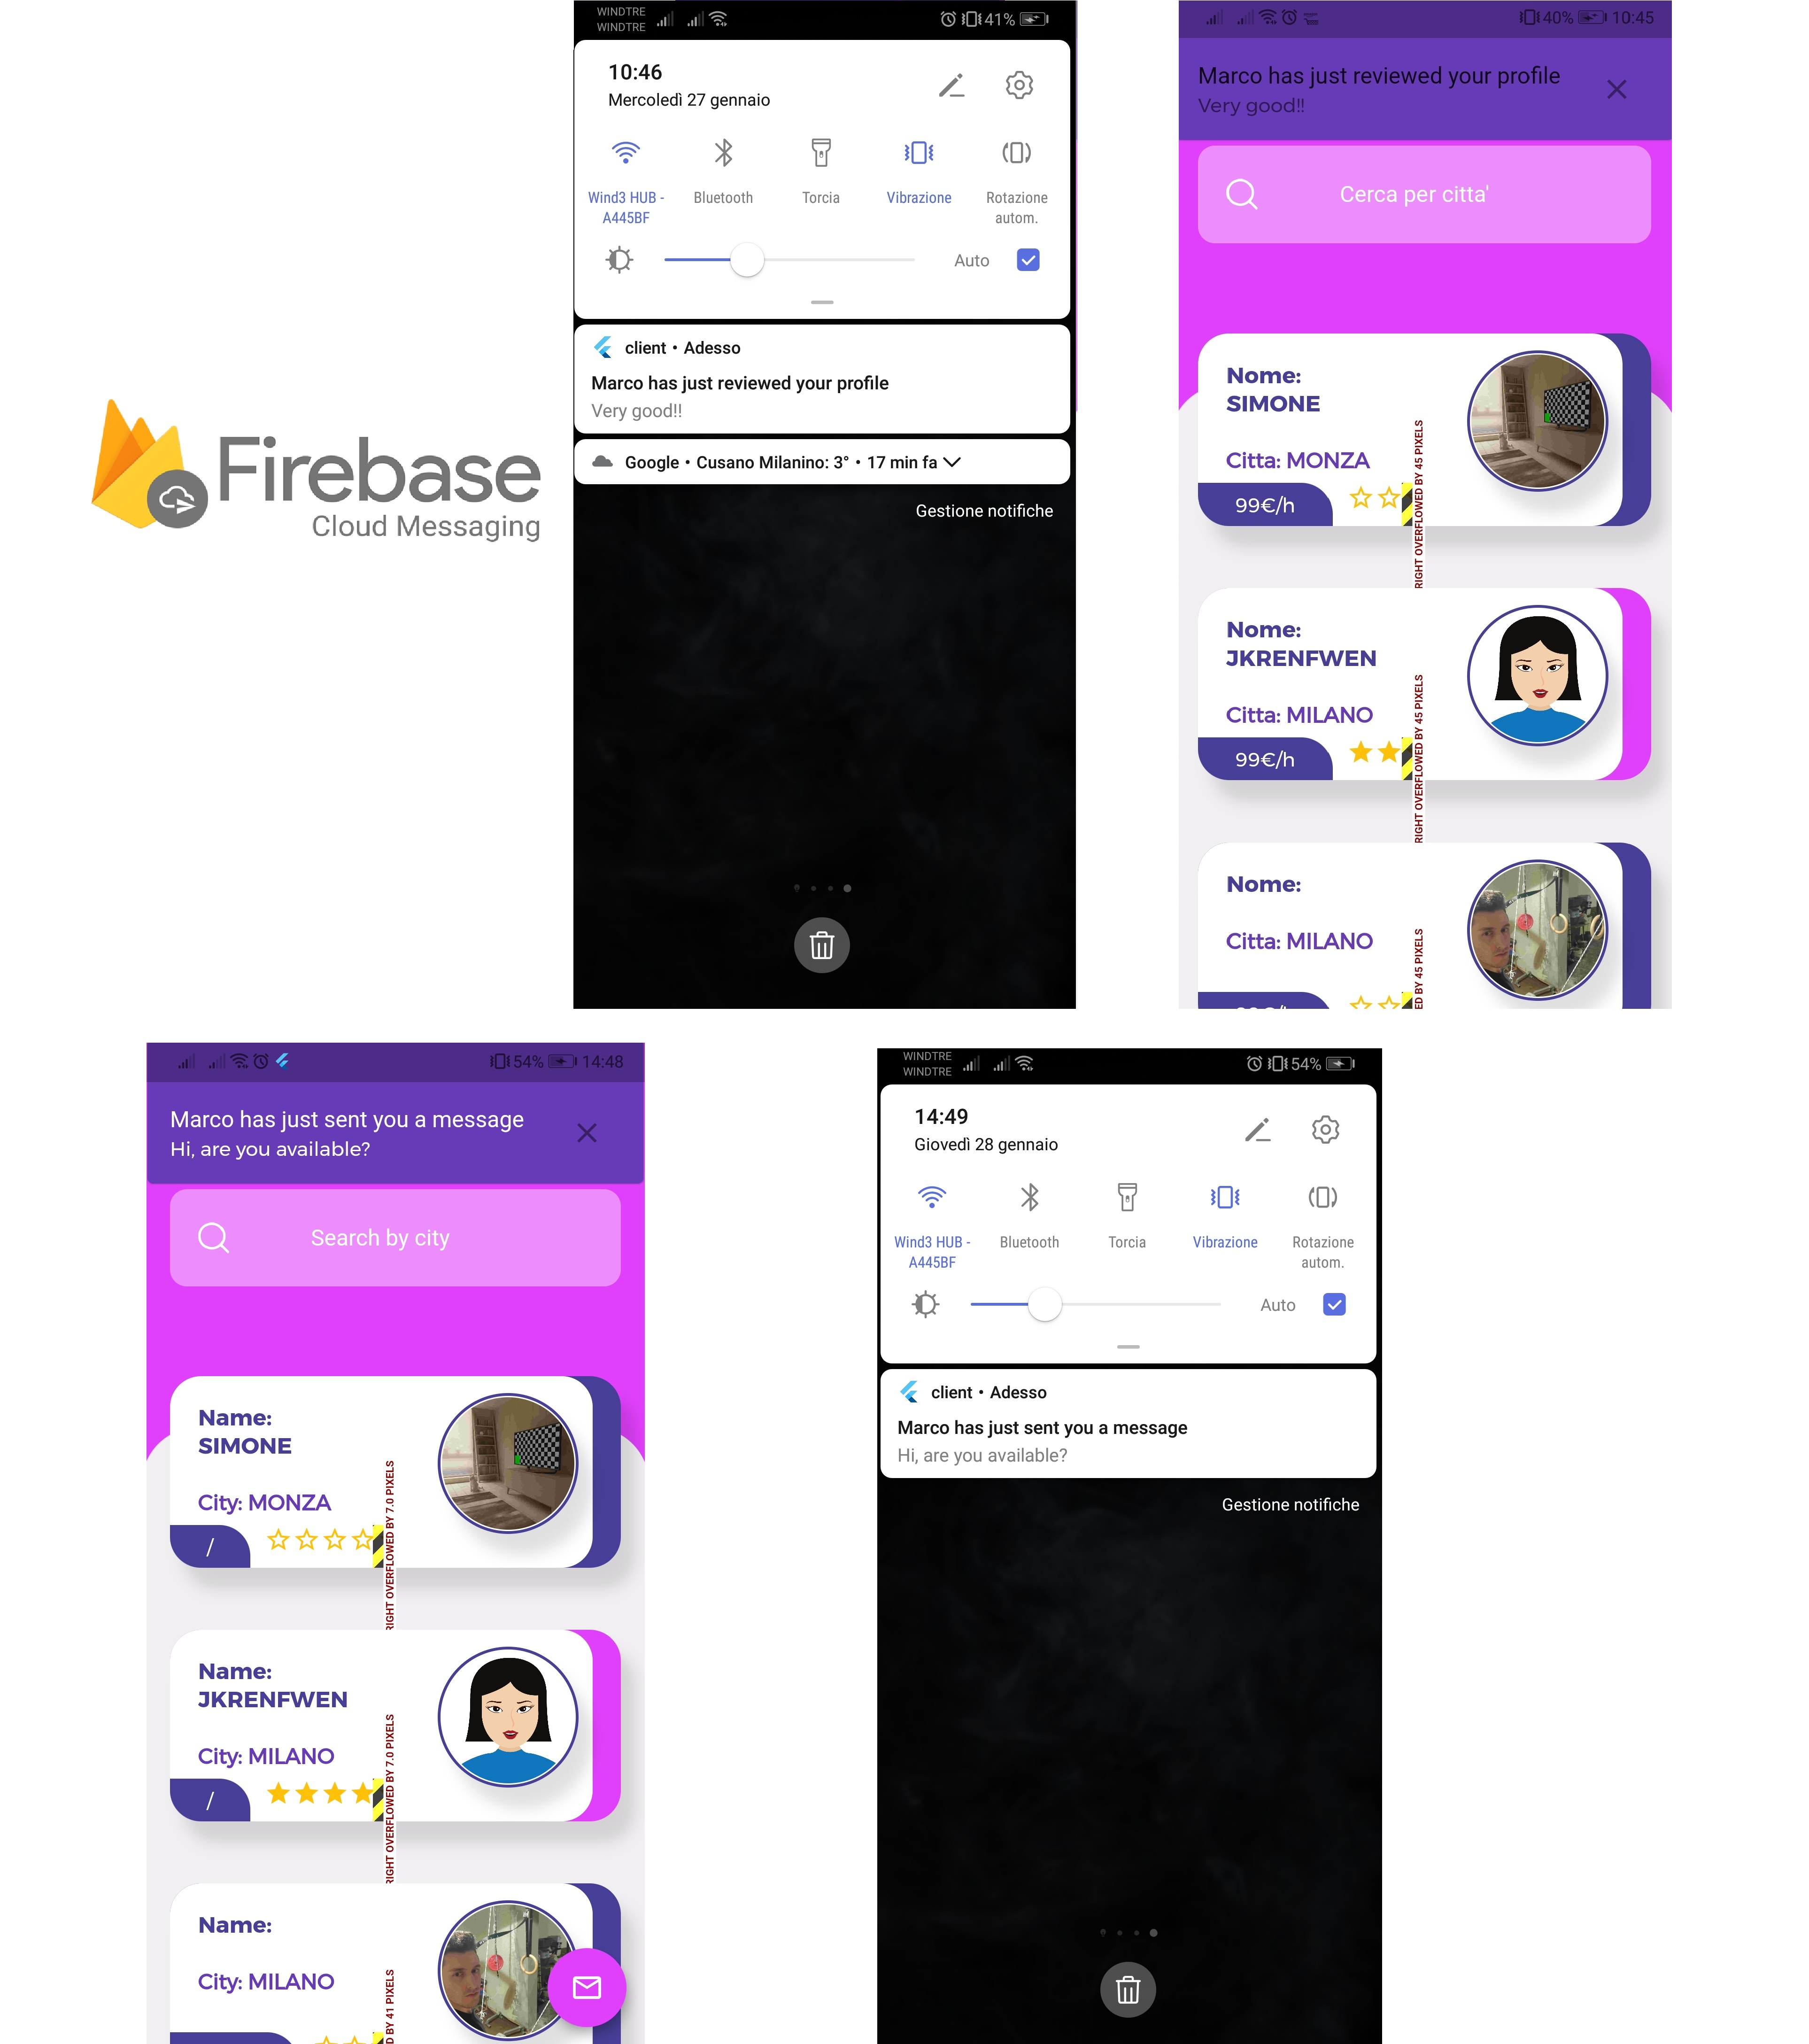
\includegraphics[scale=0.2]{../../assets/fcm.jpg}
        \caption{Background and Foreground notification of a new review}\label{fig:widget-tests}
    \end{figure}

    \newpage
    \subsection{Firebase Cloud Storage}
    Firebase Cloud Storage gives the possibility to upload and share user generated content, such as images and video, in order to build in the easiest way media content for applications. The Cloud storage is available also for Flutter; that means that files can be uploaded directly from mobile devices and web browsers. In the context of the application the service is used to upload the profile image in order to display it whenever is required.

    \begin{figure}[H]
        \centering
        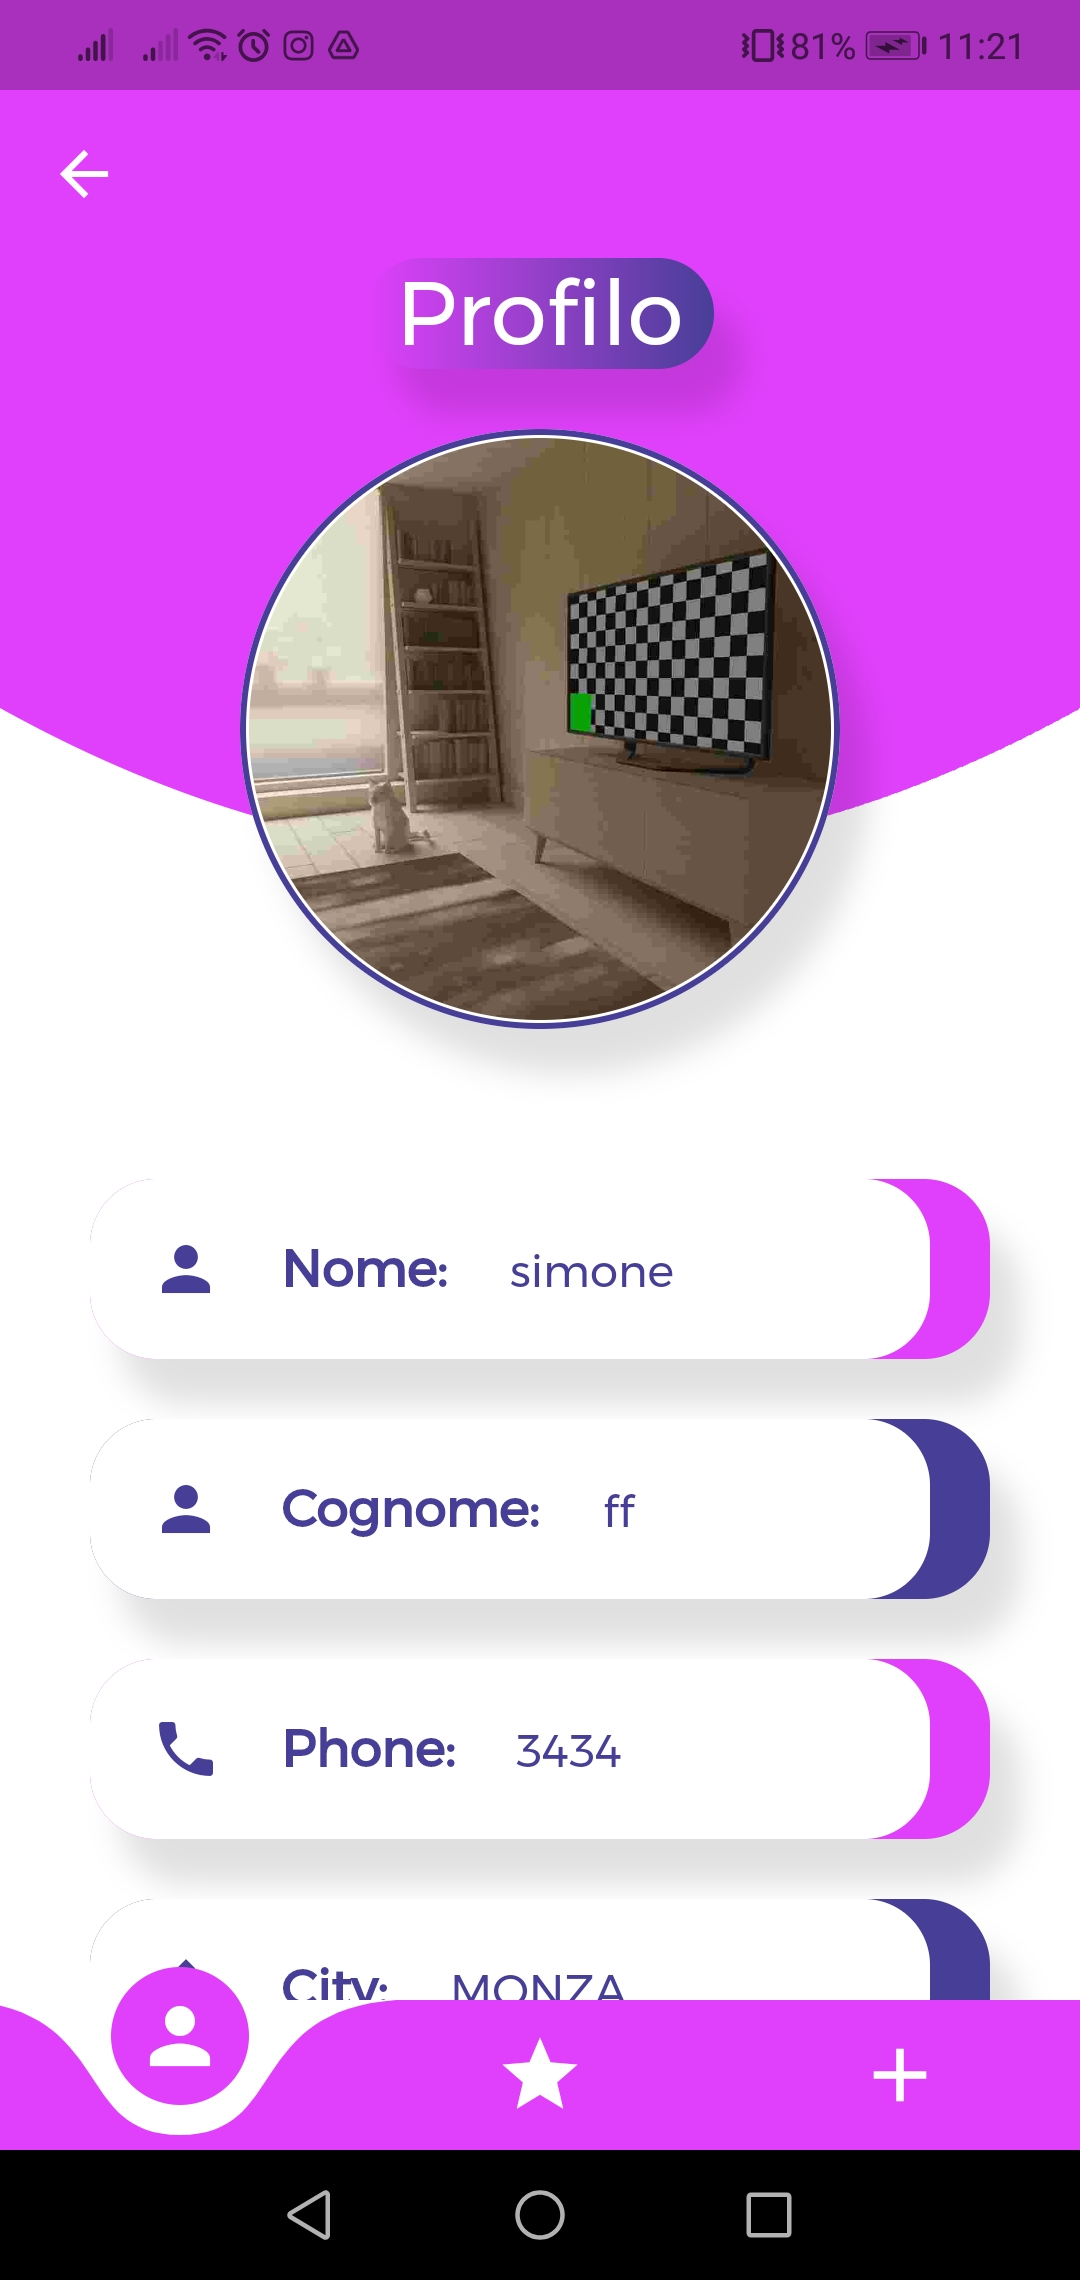
\includegraphics[scale=0.2]{../../assets/fcs.jpg}
        \caption{Profile image previously uploaded by the user via Firebase Cloud Storage}\label{fig:widget-tests}
    \end{figure}


    \section{Libraries}
    For the development of the application the majority of the libraries used are standard packages of Flutter. There are however some components that use platform SDKs to interact with external services mentioned above.

    \subsection{Firebase Messaging SDK}
    This client side component manages all the events that come with a push notification, allowing to define the behaviour of the application according to its state when a new notification is received. The fragment of code below shows how the SDK is used to define the actions to take when the app is in foreground.
    \vspace{2 mm}
    \lstinputlisting{assets/code/main.dart}
    \vspace{8 mm}

    \subsection{Firebase Storage SDK}
    In this case the SDK of Firebase is use to upload the profile image of the user and to get its reference in order to display it by simply referring to a URL. In only three lines of code we have done all the stuffs.
    \vspace{2 mm}
    \lstinputlisting{assets/code/apis.dart}
    \vspace{8 mm}

    \subsection{Other dependencies}
    In the development process of the application, we also employed the following external libraries of Flutter:

    \begin{itemize}
        \item \textbf{dio[3.0.10]}: a powerful Http client for Dart, which supports Interceptors, Global configuration and other useful features used to invoke the REST service of the server-side components;
        \item \textbf{flutter\_secure\_storage[3.3.5]}: a Flutter plugin to store data in secure storage, used to store the jwt and other sensitive information;
        \item \textbf{cupertino\_icons[1.0.0]}: asset repo containing the default set of icon assets used by Flutter's Cupertino widgets;
        \item \textbf{provider[4.3.2+2]}:  a wrapper around InheritedWidget to make them easier to use and more reusable, used for the \textbf{state management};
        \item \textbf{flutter\_spinkit[4.1.2+1]}: a collection of loading indicators animated with Flutter;
        \item \textbf{image\_picker[0.6.7+12]}: a Flutter plugin for picking images from the image library, and taking new pictures with the camera, used to upload the profile image;
        \item \textbf{awesome\_dialog[1.2.1]}: a Flutter package project for simple and awesome dialogs;
        \item \textbf{flushbar[1.10.4]}: a flexible widget for user notification that allows to customize text, button, duration and animations;
        \item \textbf{cached\_network\_image[2.3.3]}: a flutter library to show images from the internet and keep them in the cache directory, used for the profile image;
        \item \textbf{argon\_buttons\_flutter[1.0.6]}: package used to create the buttons of the application;
        \item \textbf{liquid\_swipe[1.5.0]}: a Flutter plugin to implement liquid Swipe effect to provided containers, used for the onboarding page;
        \item \textbf{google\_fonts[1.1.1]}: with  google\_fonts package, .ttf or .otf files do not need to be stored in your assets. Instead, they can be fetched once via http at runtime, and cached in the app's file system;
        \item \textbf{curved\_navigation\_bar[0.3.4]}: package used for the navigation bar;
        \item \textbf{url\_launcher[5.7.10]}: used to open the dial when tapping on profile's contact details;
        \item \textbf{toggle\_switch[0.1.8]}: used to render toggle switch widget;
        \item \textbf{font\_awesome\_flutter[8.10.0]}: icon pack available as set of Flutter Icons;
        \item \textbf{overlay\_support[1.0.5]}: support for overlay, easy to build toast and internal notification, used to render foreground notifications.
    \end{itemize}

\end{document}